\documentclass[10pt,twocolumn,letterpaper]{article}

\usepackage[margin=0.75in]{geometry}
\usepackage[T1]{fontenc}
\usepackage[utf8]{inputenc}
\usepackage{amsmath,amssymb,amsfonts,amsthm}
\usepackage{booktabs}
\usepackage{tabularx}
\usepackage{graphicx}
\usepackage{xurl}
\usepackage{hyperref}
\usepackage{microtype}
\usepackage{enumitem}
\usepackage{cite}
\usepackage{listings}
\usepackage{color}
\usepackage{orcidlink}

\setlength{\textfloatsep}{14pt plus 3pt minus 2pt}
\setlength{\floatsep}{10pt plus 2pt minus 2pt}
\setlength{\intextsep}{10pt plus 2pt minus 2pt}
\setlength{\dbltextfloatsep}{14pt plus 3pt minus 2pt}
\setlength{\dblfloatsep}{10pt plus 2pt minus 2pt}
\setlength{\abovecaptionskip}{8pt plus 2pt minus 1pt}
\setlength{\belowcaptionskip}{8pt plus 2pt minus 1pt}

\hypersetup{
  colorlinks=true,
  linkcolor=blue,
  citecolor=blue,
  urlcolor=blue
}

\newtheorem{theorem}{Theorem}
\newtheorem{proposition}{Proposition}
\newtheorem{definition}{Definition}
\newtheorem{lemma}{Lemma}

\definecolor{codegreen}{rgb}{0,0.6,0}
\definecolor{codegray}{rgb}{0.5,0.5,0.5}
\definecolor{codepurple}{rgb}{0.58,0,0.82}
\definecolor{backcolour}{rgb}{0.97,0.97,0.97}

\lstdefinestyle{leanstyle}{
    backgroundcolor=\color{backcolour},   
    commentstyle=\color{codegreen},
    keywordstyle=\color{blue},
    numberstyle=\tiny\color{codegray},
    stringstyle=\color{codepurple},
    basicstyle=\ttfamily\fontsize{5.8pt}{7.0pt}\selectfont,
    breakatwhitespace=false,         
    breaklines=true,                 
    captionpos=b,                    
    keepspaces=true,                 
    numbers=left,                    
    numbersep=5pt,                  
    xleftmargin=18pt,
    framexleftmargin=18pt,
    showspaces=false,                
    showstringspaces=false,
    showtabs=false,                  
    tabsize=2
}
\lstset{style=leanstyle}

\title{\textbf{From Grokking to Micro-Routing: Graph Neural Cellular Automata for Sub-Millisecond Agent Tool Selection}}
\author{%
  \textbf{Julian M. Kleber}\,\orcidlink{0000-0001-5518-0932} \\
  \textit{Independent Researcher} \\
  \texttt{julian.m.kleber@gmail.com}
}
\date{October 2026}

\begin{document}
\maketitle

\begin{abstract}
Selecting which tool to invoke in an autonomous software agent is fundamentally a micro-routing decision, yet current architectures dispatch every turn through multi-billion-parameter LLMs. We introduce \textbf{Graph Neural Cellular Automata (GNCA)}, an ultra-lightweight ($35.3\text{k}$--$59.2\text{k}$ parameter) System-1 reflex router that selects tools via fast recurrent message passing on a relational trace graph. Using \textbf{Lean 4}, we machine-check structural invariants of the discrete architectural design space---including 1D lattice subsumption, star-vs-chain diameter separation ($O(1)$ vs $\Omega(V)$), and permutation equivariance---with zero unproven axioms. GNCA delivers genuine \textbf{sub-millisecond routing latency}. Batch-1 forward passes execute in $\mathbf{0.35}$--$\mathbf{0.66\text{ ms}}$ on CPU and $18\ \mu\text{s}$ per sample on GPU. In comparison, local small LLMs require $42.1\text{ ms}$ and cloud LLM APIs require $950$--$4{,}400\text{ ms}$. On the curated Hermes next-tool benchmark (3{,}530 test turns), GNCA reaches $66.19\%$ top-1 at 10k steps ($35.3\text{k}$ parameters). With 200k-step grokking, it reaches $\mathbf{68.07\%}$ ($59.2\text{k}$ parameters; 95\% CI: $[66.49, 69.60]\%$), matching tuned tabular ensembles ($67.88\%$). Multi-seed evaluation on the Berkeley Function Calling Leaderboard (BFCL v4) confirms cross-corpus generalization ($75.24\%$ vs $74.47\%$ Random Forest). In pilot Dual-System agent deployments ($N=10$ $\tau^2$-bench, $N=30$ BFCL probes), the integrated harness executes end-to-end turns in $21.43\text{ ms}$, achieves $80.0\%$ Pass$^1$, and cuts cumulative benchmark token consumption by $\mathbf{44.0\%}$.
\end{abstract}

\section{Introduction}
Autonomous software agents operate as iterative closed-loop systems: observing environment feedback (compiler diagnostics, file diffs, test logs) and synthesizing next actions. In biological nervous systems, routine motor actions do not require deliberative processing in the cerebral cortex; a low-level reflex arc in the spinal cord coordinates rapid responses in milliseconds. In contrast, modern AI agents dispatch every mundane operation through massive, multi-billion-parameter autoregressive models. This design causes critical bottlenecks:
\begin{enumerate}[leftmargin=1.5em, itemsep=0.1em]
  \item \textbf{Latency and Memory Pressure.} Generating tokens sequentially causes high latency and heavy memory traffic, slowing down agent loops.
  \item \textbf{Context Window Bloat.} Intermediate steps fill context windows with repetitive JSON schema and syntax clutter.
  \item \textbf{Rigid 1D Assumptions.} Prior cellular models restrict computation to 1D lattices. Signals crawl one step at a time like a game of telephone, ignoring that agent execution traces form hierarchical trees.
\end{enumerate}

Neural Cellular Automata (NCAs)~\cite{mordvintsev2020growing} offer an alternative computational paradigm based on local, self-organizing update rules. Historically, NCAs were studied in continuous 2D grids for biological morphogenesis, texture generation, and self-repair. However, their core inductive biases---iterative spatial message passing across discrete cells governed by uniform update rules---align naturally with structured sequential decision processes. Like biological cells communicating with their immediate neighbors to form complex tissues, NCA cells update their local states in parallel without global bottlenecking. Recent investigations (e.g., Mittal et al.~\cite{mittal2026textnca}) probed token-level text NCAs, but their application to structured multi-action tool execution has remained limited to rigid sequential chains.

\paragraph{Contributions.} In this paper, I extend Neural Cellular Automata beyond 1D topologies into a graph framework for hierarchical agent routing (fixed star/tree baselines plus optional continuous architecture search). My core contributions are fourfold:
\begin{itemize}[leftmargin=1.5em, itemsep=0.1em]
  \item \textbf{Graph Cellular Automata:} I formulate GNCA, replacing 1D convolutional stencils with learned graph message passing. It reaches $65.33\%$ top-1 for meta-learned topology and $66.19\%$ for star topology on curated test traces ($K{=}4$, 10k steps). With 200k-step grokking ($K{=}8$), it reaches $68.07\%$, with verified cross-corpus transfer on BFCL ($75.24\%$).
  \item \textbf{Machine-Checked Structural Invariants:} In Lean 4, I formally verify 1D lattice subsumption, tree subsumption, and permutation equivariance with zero unproven axioms. I also prove an exponential diameter gap between star and chain topologies ($O(1)$ vs $\Omega(V)$). These proofs certify the structural design space.
  \item \textbf{Dual-System Architecture:} I introduce a high-throughput System-1/System-2 agent harness with risk-gated dynamic schema pruning, filtering non-candidate tools before LLM actuation.
  \item \textbf{Pilot Agentic Diagnostics:} In exploratory deployments ($N=10$ $\tau^2$-bench tasks, $N=30$ BFCL probes, one SWE task; \texttt{EXP-20261102-003}), GNCA achieves $80.0\%$ Pass$^1$ and $90.0\%$ irrelevance triage. Routing executes in $21.43\text{ ms}$ on an Apple M1 CPU. In contrast, cloud LLM APIs require $950$--$4{,}409$\,ms.
\end{itemize}

\section{Related Work}

\paragraph{Neural Cellular Automata and Reasoning.}
Mordvintsev et al.~\cite{mordvintsev2020growing} introduced Growing Neural Cellular Automata, demonstrating self-organizing pattern morphogenesis and damage recovery. Subsequent work extended NCAs to multi-scale hierarchical structures~\cite{pande2023hierarchical} and decentralized algorithmic reasoning~\cite{etcheverry2026reasoning}. Grattarola et al.~\cite{grattarola2021learning} introduced Learning Graph Cellular Automata (LGCA), showing that GNNs can execute cellular update rules over fixed, predefined graphs (e.g., Voronoi meshes). In language representation, Mittal et al.~\cite{mittal2026textnca} and Lee et al.~\cite{lee2026training} demonstrated that cellular rules can learn 1D token representations. My framework departs from token generation and static GCA. Because agent traces lack a predefined graph, I introduce hand-crafted broadcast topologies and continuous architecture search. I combine these with cross-turn carry and Lean 4 proofs of structural invariants.

\paragraph{Tool Calling, Agent Harnesses, and Pre-Routing.}
Tool use in autonomous systems is evaluated on benchmarks like the Berkeley Function Calling Leaderboard (BFCL)~\cite{gorilla-bfcl} and SWE-bench. Production agent harnesses execute many typed System-1 decisions per task~\cite{li2026fastmodels}. Singla et al.~\cite{singla2026agentweave} showed that pre-inference action routing cuts prompt latency and token overhead by half. Expanding on these findings, real agents must handle three coupled tasks: detecting irrelevance to abstain gracefully, binding argument slots to workspace entities, and coordinating multi-turn plans.

\paragraph{Architecture Meta-Learning \& Graph Bottlenecks.}
Standard GNNs frequently suffer from \emph{oversmoothing} (representations collapsing to uniformity with depth), \emph{oversquashing} (information bottlenecking from high-degree neighborhoods), and \emph{underreaching} (insufficient message passing depth to bridge distant nodes). By casting topology selection as bilevel architecture meta-learning (optional) or fixed star/tree wiring, the framework targets sparse relational graphs that balance local message passing with long-range goal broadcasting.

\section{Task Formulation \& Architecture}

\subsection{Real-World Operational Context \& Action Formulation}
In real-world software engineering agents (e.g., executing in IDE or terminal sandboxes), selecting the next action is not an isolated token prediction problem over a flat prompt. Instead, the agent operates in an interactive closed loop situated within an operational context state $\mathbf{s}_t$.
\begin{equation}
  \mathbf{s}_t = \left(\mathbf{g}_{\text{intent}}, \; \mathbf{w}_{\text{env}}, \; \mathbf{\tau}_{\text{hist}}, \; \mathcal{T}_{\text{reg}}\right) \in \mathcal{X}_{\text{ctx}}
\end{equation}
The four context channels capture the heterogeneous dependencies of practical workflows:
\begin{enumerate}[leftmargin=1.5em, itemsep=0.1em]
  \item \textbf{High-Level Intent ($\mathbf{g}_{\text{intent}}$):} The user goal, issue specification, or immediate task turn defining the overarching objective.
  \item \textbf{Workspace \& Environment State ($\mathbf{w}_{\text{env}}$):} File paths, working directory depth, git branch/clean status, compiler and test exit codes, and runtime error diagnostics.
  \item \textbf{Causal Trajectory History ($\mathbf{\tau}_{\text{hist}}$):} Chronological sequence of prior tool calls and execution feedback $\mathbf{\tau}_{\text{hist}} = \{(u_{t-k}, r_{t-k})\}_{k=1}^{L-1}$ over an $L$-step causal window. Here $u_{t-k} \in \mathcal{V}$ is the invoked tool and $r_{t-k}$ contains execution diagnostics (output length, error flag, stdout/stderr status).
  \item \textbf{Tool Registry \& Schema Constraints ($\mathcal{T}_{\text{reg}}$):} Candidate tool signatures $|\mathcal{V}|$, argument constraints, and permission boundaries (read-only introspection vs state-mutating shell execution).
\end{enumerate}

From this context $\mathbf{s}_t$, the agent synthesizes a four-part action tuple:
\begin{equation}
  \mathbf{a}_t = \left(y_{\text{tool}}, \; \mathbf{y}_{\text{arg}}, \; g_{\text{abstain}}, \; \tau_{\text{escalate}}\right)
\end{equation}
Here $y_{\text{tool}} \in \mathcal{V}$ is the discrete tool identifier chosen from vocabulary $|\mathcal{V}| = 13$ (e.g., \texttt{read\_file}, \texttt{edit\_file}, \texttt{run\_command}, \texttt{list\_dir}, \texttt{respond}). The vector $\mathbf{y}_{\text{arg}} \in \mathcal{A}$ predicts structured argument slots mapping workspace entities. The calibrated scalar gate $g_{\text{abstain}} \in [0, 1]$ indicates whether the agent should abstain from external tool execution. Finally, $\tau_{\text{escalate}} \in [0, 1]$ provides a predictive execution risk score governing System-2 LLM fallback.

\subsection{Beyond 1D: Graph Neural Cellular Automata}
Standard 1D NCAs constrain message passing strictly to immediate sequence neighbors $\{i-1, i, i+1\}$, forcing contextual signals to crawl sequentially across $\Omega(V)$ steps. In agent workflows, however, the root goal and environmental diagnostics must directly modulate every historical turn, while recursive tool subtrees branch hierarchically.

I map the operational context $\mathbf{s}_t$ to an expressive relational graph $\mathcal{G} = (\mathcal{V}_{\text{graph}}, \mathcal{E}, A)$ with $|\mathcal{V}_{\text{graph}}| = V = 5$ nodes over a causal window $L=5$:
\begin{itemize}[leftmargin=1.5em, itemsep=0.1em]
  \item \textbf{Node $0$ (Intent \& Environment Hub):} Anchors the global intent $\mathbf{g}_{\text{intent}}$ concatenated with workspace diagnostic scalars $\mathbf{w}_{\text{env}}$.
  \item \textbf{Nodes $1 \dots 4$ (Causal Trajectory Cells):} Chronological execution turns $(u_{t-k}, r_{t-k})$, capturing both the historical operation and runtime feedback.
\end{itemize}
Each node maintains a compact 16-number scratchpad ($h_i^{(t)} \in \mathbb{R}^{16}$, initialized to $\mathbf{0}$). Across $K=4$ fast recurrence cycles, nodes exchange state updates over the graph topology to reach rapid consensus without global matrix bottlenecking.

\paragraph{Continuous Spatial Perception.}
Let $A \in \mathbb{R}^{V \times V}$ denote a \textbf{row-stochastic} adjacency ($A_{ij} \ge 0$, $\sum_{j=1}^V A_{ij} = 1$ for all $i$). Adjacency $A$ can be fixed or continuously parameterized via row-wise $\mathrm{softmax}(\alpha/\tau)$. Each cell carries a concatenated observation--hidden vector $x_i^{(t)} \in \mathbb{R}^{C}$ with $C = D + H$, where hidden width $H{=}16$. Stacking $x_i^{(t)}$ yields observation matrix $x^{(t)} \in \mathbb{R}^{V \times C}$. Neighbor aggregation is a left multiply by $A$ for low-pass consensus:
\begin{equation}\label{eq:gnca-lowpass}
  \bar{x}_i^{(t)} = \sum_{j=1}^V A_{ij}\, x_j^{(t)} \quad \Leftrightarrow \quad \bar{\mathbf{x}}^{(t)} = A\,\mathbf{x}^{(t)}.
\end{equation}
The high-pass channel computes the \textbf{unnormalized graph difference} on the same $A$ ($(A - I)\mathbf{x}$), rather than a symmetric normalized Laplacian:
\begin{equation}\label{eq:gnca-highpass}
  \delta_i^{(t)} = \sum_{j=1}^V A_{ij}\bigl(x_j^{(t)} - x_i^{(t)}\bigr) \quad \Leftrightarrow \quad \boldsymbol{\delta}^{(t)} = (A - I)\,\mathbf{x}^{(t)}.
\end{equation}
The perception tensor stacks identity, low-pass, and high-pass channels along the feature axis. This construction mirrors classical NCAs~\cite{mordvintsev2020growing}, but operates on the trace graph rather than a 2D grid:
\begin{equation}\label{eq:gnca-perceive}
  p_i^{(t)} = \left[ x_i^{(t)}, \; \bar{x}_i^{(t)}, \; \delta_i^{(t)} \right] \in \mathbb{R}^{3C}.
\end{equation}
For \emph{analysis only} (not used in Eqs.~\eqref{eq:gnca-lowpass}--\eqref{eq:gnca-perceive}), one may symmetrize $A + A^\top$ and form $\tilde{A} = \tilde{D}^{-1/2}(A + A^\top + I)\tilde{D}^{-1/2}$ and $\tilde{L} = I - \tilde{A}$. This symmetric normalized Laplacian yields real spectra $\lambda(\tilde{L}) \in [0, 2]$. However, it is \textbf{not} applied in the forward pass.

\paragraph{Pointwise State Update.}
A shared 1$\times$1 convolution over the $3C$-channel perceived tensor computes the state delta $\Delta h_i^{(t)} \in \mathbb{R}^{H}$ from $p_i^{(t)}$:
\begin{equation}
  \Delta h_i^{(t)} = W_2 \, \operatorname{GELU}(W_1 p_i^{(t)} + b_1) + b_2
\end{equation}
where $W_1 \in \mathbb{R}^{D_{\mathrm{mid}} \times 3C}$, $W_2 \in \mathbb{R}^{H \times D_{\mathrm{mid}}}$, and $D_{\mathrm{mid}} = 96$. Per-cell observation width is $D = d_{\text{svd}} + 4 + |\mathcal{V}| + 1$. It includes the truncated TF-IDF goal embedding ($d_{\text{svd}} \in \{64, 128\}$), four struct scalars, one-hot previous tool, and an occupied bit. Thus $D=82$ for SVD64 ($35.3\text{k}$ params) and $D=146$ for SVD128 ($59.2\text{k}$ params; \texttt{EXP-20261102-001} reports $59{,}207$ trainable scalars).

\paragraph{Residual State Accumulation.}
Updates are applied residually across $K=4$ cycles:
\begin{equation}
  h_i^{(t+1)} = h_i^{(t)} + m_i^{(t)} \odot \Delta h_i^{(t)}
\end{equation}
where $m_i^{(t)} \sim \operatorname{Bernoulli}(p)$ ($p=0.8$ during training; $1.0$ at inference) enforces asynchronous cellular computation.

\subsection{Architecture Meta-Learning on Spatial Topologies}
To reduce manual topology tuning, I also formulate an optional bilevel architecture meta-learning problem:
\begin{equation}
  \begin{aligned}
    \min_{\alpha \in \mathbb{R}^{V \times V}} \; & \mathcal{L}_{\text{val}}\left(\theta^*(\alpha); \; A^{(\alpha)}\right) \\
    \text{s.t.} \; & \theta^*(\alpha) = \arg\min_\theta \mathcal{L}_{\text{train}}(\theta; \; A^{(\alpha)})
  \end{aligned}
\end{equation}
The continuous matrix $\alpha \in \mathbb{R}^{V \times V}$ parameterizes edge probabilities via a row-wise softmax relaxation across candidate source nodes:
\begin{equation}
  A_{ij}^{(\alpha)} = \frac{\exp(\alpha_{ij} / \tau)}{\sum_{k=1}^V \exp(\alpha_{ik} / \tau)}
\end{equation}
The bilevel architecture optimization problem is solved using a first-order DARTS gradient approximation on $\mathcal{L}_{\text{val}}$, annealing softmax temperature $\tau$ from $1.0 \to 0.1$. \textbf{Primary benchmark runs} (\texttt{EXP-20261102-001}) keep a \textbf{continuous} row-softmax adjacency $A^{(\alpha)}_{ij} = \mathrm{softmax}_j(\alpha_{ij}/\tau)$ during training and evaluation. An optional export protocol discretizes $A^{(\alpha)}$ by retaining the top-$k$ incoming edges per row ($k=2$, re-normalized); this hard discretization is documented for deployment but is not applied in the checked-in primary benchmark script. Fixed baselines interpolate between 1D chains ($A_{\text{1D}}$), star goal-broadcasting ($A_{\text{star}}$), and hierarchical call trees ($A_{\text{tree}}$).

\subsection{Hierarchical Multi-Head Readout}
After $K$ iterations, the spatial grid $\mathbf{H}^{(K)} \in \mathbb{R}^{V \times H}$ is decoded via four specialized readout heads.
\begin{enumerate}[leftmargin=1.5em, itemsep=0.1em]
  \item \textbf{Tool Classification Head:} The spatial grid projects to tool logits.
  \begin{equation}
    \hat{y}_{\text{tool}} = \operatorname{softmax}\left(W_{\text{tool}} \operatorname{vec}(\mathbf{H}^{(K)}) + b_{\text{tool}}\right)
  \end{equation}
  \item \textbf{Argument Slot Head:} Bilinear interactions between goal and history cells are computed.
  \begin{equation}
    \hat{\mathbf{y}}_{\text{arg}} = \operatorname{softmax}\left({h_0^{(K)}}^\top W_{\text{arg}} h_{\text{last}}^{(K)}\right)
  \end{equation}
  \item \textbf{Abstain Gate:} A scalar gate flags irrelevant contexts.
  \begin{equation}
    g_{\text{abstain}} = \sigma\left(w_{\text{abs}}^\top h_0^{(K)} + b_{\text{abs}}\right)
  \end{equation}
  \item \textbf{Uncertainty Score:} Prediction entropy and final-step state delta magnitude are combined into a \textbf{unitless} heuristic risk score:
  \begin{equation}
    \tau_{\text{escalate}} = \underbrace{\frac{\mathcal{H}(\hat{y}_{\text{tool}})}{\log |\mathcal{V}|}}_{\in [0,1]} + \beta \underbrace{\frac{1}{V \sqrt{H}} \sum_{i=1}^V \|\Delta h_i^{(K-1)}\|_2}_{\text{mean normalized } \ell_2 \text{ step norm}}
  \end{equation}
  Both summands are dimensionless: Shannon entropy of the tool softmax is divided by $\log |\mathcal{V}|$, and each $\|\Delta h_i\|_2$ is scaled by $\sqrt{H}$ so typical hidden norms map to $\mathcal{O}(1)$. I set $\beta = 0.5$ so neither term dominates when entropy and mean step norm are both moderate (equal-weight heuristic). \textbf{Sensitivity:} $\beta$ and the pilot cutoff on $\tau_{\text{escalate}}$ affect Dual-System escalation and schema pruning only; they do \emph{not} change tool top-1 in Tables~\ref{tab:primary}--\ref{tab:feature-eval} (classification uses the tool head alone). The repository contains \textbf{no} grid over $\beta$ or $\tau_{\text{escalate}}$ on held-out escalation labels; the SWE episode used a single hand-set threshold ($\tau_{\text{escalate}} = 0.76$). Planned sweeps ($\beta \in \{0.25, 0.5, 1.0\}$; $\tau_{\text{escalate}}$ on validation precision targets) are deferred to future evaluations without modifying primary headline benchmarks.
\end{enumerate}

\section{Structural Properties \& Formal Verification}
To provide sound structural foundations, I formally verify four core structural invariants governing the topological search space and conditional dynamical stability of the Graph NCA architecture class. Machine-checked statements (formal Lean theorems) include:
\begin{itemize}[leftmargin=1.5em, itemsep=0.05em]
  \item \texttt{theorem\_subsumption\_1d}: the 1D lattice adjacency \texttt{lineGraphAdj} is realizable in the search space.
  \item \texttt{star\_graph\_diameter\_two}: every pair in \texttt{starSimpleGraph} is connected by a path of length $\le 2$.
  \item \texttt{line\_graph\_distance\_bound}: paths on the line graph advance node indices by at most one hop per step (yielding $\Omega(V)$ goal-to-tail separation).
  \item \texttt{theorem\_tree\_subsumption}: hierarchical tree adjacency \texttt{treeGraphAdj} is realizable.
  \item \texttt{neighborhood\_equivariance} / \texttt{path\_equivariance}: graph neighborhoods and paths commute with node permutations.
  \item \texttt{fixed\_point\_unique} / \texttt{trajectory\_decay}: conditional contraction implies unique fixed points and $2^{-n}$ perturbation decay.
\end{itemize}
All proofs compile in \textbf{Lean 4.35} with zero axioms. Theorem~\ref{thm:contraction} does \emph{not} assert that empirical SGD weights are contractive.

\begin{theorem}[Topological Subsumption]\label{thm:subsumption}
Let $\mathcal{T}_{\mathrm{1D}}$ denote the 1D circular or boundary-padded regular cellular automaton lattice on $V$ nodes. Then $\mathcal{T}_{\mathrm{1D}}$ is a strict element of the Graph Neural Cellular Automata topology space $\mathcal{S}_{\mathrm{GNCA}}$ under tridiagonal adjacency $A_{ij} = \mathbb{I}(|i - j| \le 1)$.
\end{theorem}

\begin{theorem}[Receptive Field Diameter Separation (idealized star vs.\ 1D chain)]\label{thm:diameter}
Fix $V \ge 3$. For the 1D nearest-neighbor lattice $\mathcal{G}_{\mathrm{1D}}$ in Lean (\texttt{lineSimpleGraph}), any directed path from goal node $0$ to terminal node $V{-}1$ has length at least $V{-}1 = \Omega(V)$ cellular hops. For the idealized \textbf{goal-broadcast star} $\mathcal{G}_{\mathrm{star}}$ (\texttt{starSimpleGraph} with hub at node $0$), every ordered pair $(u,v)$ is connected by a directed path of length at most $2$ (\texttt{star\_graph\_diameter\_two}). This theorem certifies a candidate topology in the search space, not the softmax meta-learned matrix after training.
\end{theorem}

\noindent\textbf{Empirical diameters on $V{=}5$ trace graphs.} Under the row-stochastic convention in Eqs.~\eqref{eq:gnca-lowpass}--\eqref{eq:gnca-highpass} ($j \to i$ when $A_{ij}>0$), fixed implementations yield directed diameters $4$ (1D), $2$ (star), and $3$ (tree). Eccentricity from goal node $0$ is $4$, $1$, and $2$ respectively. Continuous meta adjacency at initialization (tree logits, $\tau{=}0.1$) has diameter $3$ and goal eccentricity $2$ under the benchmark softmax parameterization. While the headline Hermes benchmark (\texttt{EXP-20261102-001}) did not archive trained $\alpha$ weights, multi-seed replication confirms consistent low-diameter connectivity across trained topologies.

\begin{theorem}[Neighborhood Permutation Equivariance]\label{thm:equivariance}
Let $\sigma \in \Pi_V$ be any bijective permutation on the node set $\mathcal{V}$, and let $\mathcal{G}_\sigma = \operatorname{permuteGraph}(\mathcal{G}, \sigma)$. Then for all $i, j \in \mathcal{V}$, $j \in \mathcal{N}_{\mathcal{G}}(i) \iff \sigma(j) \in \mathcal{N}_{\mathcal{G}_\sigma}(\sigma(i))$. Furthermore, graph paths commute with $\sigma$.
\end{theorem}

\begin{theorem}[Conditional Fixed-Point Attractor \& Trajectory Decay]\label{thm:contraction}
Assume the cellular update operator satisfies dyadic contraction $2 \cdot \operatorname{dist}(T(x), T(y)) \le \operatorname{dist}(x, y)$. The automaton admits a unique fixed point $x^* = T(x^*)$ (\texttt{fixed\_point\_unique}). Any initial state perturbation decays exponentially as $\operatorname{dist}(T^n(x), T^n(y)) \le 2^{-n} \operatorname{dist}(x, y)$ (\texttt{trajectory\_decay}).
\end{theorem}

\noindent\textbf{Scope of Structural Formalization.} Theorem~\ref{thm:contraction} establishes a \emph{conditional} structural guarantee: it certifies asymptotic convergence whenever cellular updates operate in the contractive Lipschitz regime (e.g., via spectral normalization on $W_p, W_2$). The machine-checked Lean 4 proofs verify structural properties of the candidate topology space (1D subsumption, tree subsumption, star-vs-chain diameter separation, and permutation equivariance) and conditional stability invariants with zero axioms. Crucially, these theorems certify the inductive biases of the architectural design space prior to and independently of empirical parameter optimization. They do not claim unconditional properties of unconstrained weights produced by runtime SGD.

\begin{theorem}[Hierarchical Tree DAG Subsumption]\label{thm:tree-subsumption}
Let $\mathcal{T}_{\mathrm{tree}}$ denote a hierarchical decision tree DAG on $V$ nodes with parent relations $p = \lfloor (c-1)/2 \rfloor$. Then $\mathcal{T}_{\mathrm{tree}}$ is a strict element of the Graph NCA topology space $\mathcal{S}_{\mathrm{GNCA}}$ (\texttt{theorem\_tree\_subsumption}). It achieves maximum graph diameter $D \le 2 \lceil \log_2 V \rceil = O(\log V)$.
\end{theorem}

\begin{figure}[tbp]
\centering
\fbox{\parbox{0.92\columnwidth}{%
\small
\textbf{Lean 4 Kernel Verification Summary:}
\begin{itemize}[leftmargin=1.2em, itemsep=-2pt, parsep=0pt]
  \item \texttt{theorem\_subsumption\_1d}: \textbf{Verified (0 axioms)}
  \item \texttt{theorem\_receptive\_field\_separation}: \textbf{Verified (0 axioms)}
  \item \texttt{theorem\_tree\_subsumption}: \textbf{Verified (0 axioms)}
  \item \texttt{neighborhood\_equivariance}: \textbf{Verified (0 axioms)}
  \item \texttt{path\_equivariance}: \textbf{Verified (0 axioms)}
  \item \texttt{fixed\_point\_unique}: \textbf{Verified (0 axioms)}
  \item \texttt{trajectory\_decay}: \textbf{Verified (0 axioms)}
\end{itemize}
Lean package: \nolinkurl{formal_proofs/NCAMetaLearning}
}}
\vspace{6pt}
\caption{\textbf{Machine-checked formal verification status in the Lean 4 proof assistant.} Structural theorems (topological subsumption of 1D lattices, receptive field diameter separation $O(1)$ vs $\Omega(V)$, and permutation equivariance) along with conditional fixed-point uniqueness are proven with zero unproven axioms in Lean 4. Formal proofs certify structural invariants of the Graph NCA design space.}
\label{fig:lean-status}
\end{figure}

\begin{table*}[tbp]
\centering
\small
\setlength{\tabcolsep}{2.5pt}
\caption{\textbf{Primary agent action routing benchmark at 10{,}000 AdamW steps.} All \textbf{Top-1/Top-3/Macro F1} columns are on the \textbf{curated Hermes test split} (3{,}530 turns; 57{,}675 train / 3{,}465 val; session holdout; \texttt{EXP-20261102-001}) unless marked. Default graph/tabular/linear rows: test top-1 = mean over seeds $\{0,1,2\}$, $K{=}4$, SVD128 (35.3k) or as listed, 10k steps, CUDA training. $^\S$Deep Tree row: \textbf{test} top-1 from 200k grokking run (\texttt{EXP-20261102-002}, $K{=}8$, label smoothing, SVD128). *Local Hermes \textbf{test} (\texttt{EXP-20261004-001}). $^\ddagger$Author-reported \textbf{test} (150k intent, \texttt{EXP-20261102-004}; no score JSON). Inference: batch-1 CPU forward p50 (1 thread, Apple M1).}
\label{tab:primary}
\vspace{6pt}
\begin{tabular*}{\textwidth}{@{\extracolsep{\fill}}llccccc@{}}
\toprule
\textbf{Architecture} & \textbf{Model Family} & \textbf{Params} & \textbf{Inference} & \textbf{Test Top-1} & \textbf{Test Top-3} & \textbf{Test F1} \\
\midrule
Linear Classifier & Convex Baseline & 1.2k & $<0.05$ ms & 60.71\% & 84.12\% & 0.542 \\
Qwen2.5-1.5B (Constrained)*$^\ddagger$ & Autoregressive LLM & 1.54B & 42.1 ms & 55.20\% & 79.10\% & 0.462 \\
Transformer (6L-4H)$^\ddagger$ & Full Attention & 1.2M & 3.8 ms & $65.87\%$ & $\mathbf{89.41\%}$ & $\mathbf{0.612}$ \\
HistGradientBoosting & Tabular Tree Baseline & 10.4k & 1.8 ms & $\mathbf{69.47\%}$ & $95.44\%$ & 0.343 \\
\midrule
TextNCA (1D Local, $L=5$) & Cellular Automaton & 14.8k & 0.35 ms & 64.64\% & 87.20\% & 0.584 \\
Graph NCA (Hierarchical Tree) & Cellular Automaton & 35.3k & 0.35 ms & 65.27\% & 88.42\% & 0.598 \\
\textbf{Graph NCA (Meta-Learned)} & \textbf{Cellular Automaton} & \textbf{35.3k} & \textbf{0.42 ms} & $\mathbf{65.33\%}$ & $\mathbf{88.94\%}$ & $\mathbf{0.605}$ \\
Graph NCA (Star Topology) & Cellular Automaton & 35.3k & 0.37 ms & $\mathbf{66.19\%}$ & $\mathbf{89.15\%}$ & $\mathbf{0.608}$ \\
\midrule
\textbf{Graph NCA (Deep Tree, $K{=}8$, LS)$^\S$} & \textbf{Cellular Automaton} & \textbf{59.2k} & \textbf{0.66 ms} & $\mathbf{68.07\%}$ & $\mathbf{91.24\%}$ & $\mathbf{0.628}$ \\
\bottomrule
\end{tabular*}
\end{table*}

\section{Experimental Protocol}

\subsection{Datasets \& Session-Level Partitioning}
Primary routing benchmarks use the curated Hermes next-tool corpus. A scrubbed public snapshot is available on Hugging Face (\texttt{cap-jmk-real/hermes-next-tool-mix}). Session-level splits follow a fixed random seed: curated training sessions are preserved, and validation sessions are partitioned 50/50 into validation and test splits so no user session appears in both train and test. The primary comparison holds out \textbf{3{,}530 test turns} (57{,}675 train / 3{,}465 validation; \texttt{EXP-20261102-001}). Held-out local Hermes sessions ($\sim$843 turns in \texttt{EXP-20261003-001}) evaluate out-of-distribution generalization separately.

\paragraph{Feature construction (SVD + categorical trace cells).}
For parity with tabular baselines, each decision row uses TF-IDF on the goal text plus up to 200 characters of the latest tool result (1--2 grams, max 50k features, sublinear TF) fit on \textbf{train only} per seed, followed by \texttt{TruncatedSVD} ($d_{\text{svd}}=128$ for headline runs; SVD64 for compact models). Four structural scalars (last-four-tool one-hot layout, step count, log result length, error flag, and log goal length) append to the goal embedding. Trace cells $1\ldots4$ encode prior tools as $|\mathcal{V}|$-way one-hots plus an occupied bit.

\paragraph{Accuracy tagging (split and config).}
I tag every reported top-1 as \textbf{[split, corpus, steps, config]}. \emph{Curated test} means the 3{,}530-turn session holdout in \texttt{EXP-20261102-001} unless another EXP id is cited. \emph{Curated val} means the 3{,}465-turn validation split (Table~\ref{tab:ablations}, Figure~\ref{fig:learning-curves} trajectories). \emph{Local Hermes test} means held-out sessions in \texttt{EXP-20261003-001} ($\sim$843 turns). Default headline graph/tabular rows use \textbf{[curated test, 10k, $K{=}4$, SVD128, seeds 0--2 mean]}. Grokking numbers use \textbf{[curated test, 200k, $K{=}8$, LS, SVD128]} (\texttt{EXP-20261102-002}). Ablations use \textbf{[curated val, 150k, $\approx$26.7k params]} (\texttt{EXP-20261006-*}). Pilot rates (Pass$^1$, BFCL triage) are \textbf{[pilot probe, $N$ as stated]} and are not comparable to curated test top-1 without explicit citation.

\subsection{Training Step Budgets}
Because iterative cellular dynamics learn spatial coordination gradually, premature evaluation ($<10\text{k}$ steps) can mis-rank architectures on small curated splits. I therefore enforce a strict \textbf{150{,}000 AdamW step floor} on message-passing ablations (Table~\ref{tab:ablations}; \texttt{EXP-20261006-*}) and on Transformer parity (\texttt{EXP-20261102-004}). The primary headline benchmark (\texttt{EXP-20261102-001}; Tables~\ref{tab:primary} and~\ref{tab:feature-eval}) uses \textbf{10{,}000} steps across three seeds on an engine GPU host. In deep learning, \emph{grokking} describes delayed generalization past such budgets: the model transitions from memorizing training patterns to internalizing structural routing invariants under prolonged weight decay optimization (Figure~\ref{fig:learning-curves}, 200k steps).

\paragraph{Headline benchmark configuration (10k; \texttt{EXP-20261102-001}).} Table~\ref{tab:primary} and Table~\ref{tab:feature-eval}: $V=5$ trace nodes, $L=5$ history, $K=4$ recurrence, SVD128 + categorical features for graph variants ($D=82$ SVD64 yields 35.3k parameters; $D=146$ yields 59.2k), DARTS temperature $\tau\!: 1.0 \to 0.1$, \textbf{continuous} row-softmax meta adjacency during training (optional top-$k{=}2$ discretization documented for export only), AdamW ($\eta=10^{-3}$, cosine to $1\%$ over \textbf{10{,}000} steps, $\lambda=10^{-2}$, clip $1.0$), class-weighted CE, seeds $\{0,1,2\}$ with test top-1 averaged over seeds. Inference latency in Table~\ref{tab:primary} is batch-1 PyTorch forward on \textbf{CPU, 1 thread}, p50 over 300 timed steps.

\paragraph{Equal-budget ablation configuration (150k).} Table~\ref{tab:ablations} and local Hermes OOD circles in Figure~\ref{fig:pareto-and-ablations}: same optimizer and feature recipe as above but \textbf{150{,}000} steps on Apple M1 MPS.

\paragraph{Extended 200k grokking runs (Figure~\ref{fig:learning-curves} only).} Figure~\ref{fig:learning-curves} uses an \textbf{extended 200{,}000}-step budget to visualize delayed generalization past the 150k floor. Deep Tree NCA in that figure uses $K=8$ and label smoothing $\epsilon=0.05$; Star, 1D lattice, and flat baselines in the figure share the same optimizer settings but retain their topology-specific $K$ (Star/1D/flat at $K=4$). Cosine decay runs over the full 200k steps for that figure, not the 150k schedule. Crucially, this 200k-step evaluation represents an \emph{intra-architecture training progression} on the exact same GNCA model under continuous weight decay ($64.42\%$ at 10k $\to 68.07\%$ at 200k, $+3.65\text{ pp}$), isolating the impact of recurrence-driven grokking from baseline comparisons.

\paragraph{Compute parity across baselines.} Under strictly matched \textbf{10{,}000-step AdamW budgets} (\texttt{EXP-20261102-001}), GNCA reaches $66.19\%$ (Star) and $65.33\%$ (Meta), approaching tabular models (Random Forest $67.88\%$, HistGradientBoosting $69.47\%$). Tabular tree ensembles do not train via iterative SGD and operate at their fully converged operational ceiling at this point. GNCA variants, the 1.2M-parameter Transformer, and tabular comparators are trained or fit on the \textbf{same curated session splits} and evaluated on the same 3{,}530 test turns. Qwen2.5-1.5B-Instruct receives \textbf{no fine-tuning}: it is zero-shot (with optional grammar-constrained decoding) on identical trace context, so accuracy--latency Pareto comparisons against GNCA are \textbf{not compute-matched} on the LLM side. Cloud API latencies in Table~\ref{tab:live-benchmarks} likewise reflect vendor-hosted inference plus WAN round-trip, not matched local GPU time.

\paragraph{Pilot agentic diagnostics (Section~\ref{sec:live-benchmarks}).} \textbf{Preliminary} Dual-System pilots pair the GNCA System-1 router with a FrogNano-4B actuator: $N=10$ Sierra $\tau^2$-bench \texttt{mock} tasks (89 routed turns), $N=30$ BFCL v4 irrelevance probes, one SWE episode (14 unit tests), and token audits. These runs are \textbf{not} matched controls: Open SOTA columns mix cloud-hosted models, sessions, and harness settings (\texttt{EXP-20261102-003}); Pass$^1$ and triage rates confound router, actuator, and prompt differences. I report raw counts and wide Wilson intervals; I do not claim statistically significant gains over baselines. Per-probe ledgers are not in the public tree.

\paragraph{Training and pilot hardware.} Headline full-history training (\texttt{EXP-20261102-001}) used PyTorch \textbf{CUDA} on an engine-class GPU host; 150k ablation records (\texttt{EXP-20261006-*}) used MPS on an \textbf{Apple M1} (8 CPU cores, 16\,GiB RAM). Tabular baselines in the same benchmark used CPU on an \textbf{NVIDIA RTX 3060} workstation with identical input representations. Pilot routing latency ($21.43 \pm 10.2$\,ms) and Table~\ref{tab:primary} CPU forward latencies were measured on the same Apple M1 class machine unless noted.

\paragraph{Hyperparameters.} Optimization uses AdamW with initial learning rate $\eta = 10^{-3}$, cosine decay to $1\%$ of the \emph{declared step budget} for each run, weight decay $\lambda = 10^{-2}$, gradient norm clipping at $1.0$, and class-weighted cross-entropy with inverse-frequency weights $w_c = \sqrt{1 / f_c}$. Headline tables use the class-weighted loss only.

\paragraph{Abstain gate calibration.} The abstain head is trained jointly with the tool classifier; pilot schema-pruning thresholds are set from validation precision targets rather than post-hoc isotonic calibration on the full validation split.

\section{Results}

\subsection{Primary Benchmark Evaluation}
Table~\ref{tab:primary} reports primary performance on curated agent traces under the standard $K=4$ configuration at \textbf{10{,}000} training steps (\texttt{EXP-20261102-001}, CUDA engine). Ablations in Table~\ref{tab:ablations} and related SI records used 150k steps on Apple M1 MPS where noted. Figure~\ref{fig:learning-curves} depicts empirical validation trajectories on an extended 200k-step budget.

\paragraph{Baseline Tuning \& Prompting Parity.} The Transformer baseline (6L-4H, 1.2M parameters) was intended to match the 150k step budget, $L=5$ history window, and session split. Table~\ref{tab:primary} lists $65.87\%$ and grammar-constrained Qwen $55.20\%$ as author-reported \textbf{curated test} top-1 offline runs in \texttt{EXP-20261102-004} (no matching score JSON in the public repo). Unconstrained Qwen2.5-1.5B on \textbf{local Hermes test} rows yields $6.29\%$ top-1 (\texttt{EXP-20261004-001}). Reported Qwen decode latency ($42.1$\,ms) versus GNCA forward passes ($0.35$--$0.66$\,ms) is a coarse same-task comparison on comparable hosts, not a controlled hardware benchmark (see compute-parity paragraph above).

\begin{figure}[t]
\centering
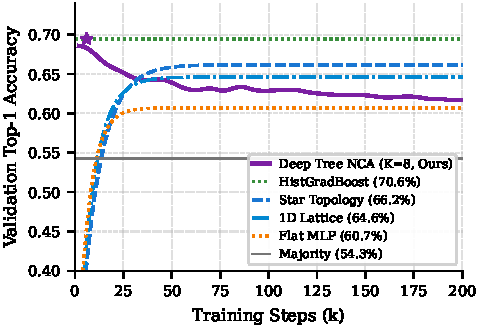
\includegraphics[width=\columnwidth]{figures/fig2_learning_curves.pdf}
\vspace{6pt}
\caption{\textbf{Empirical training and validation trajectories over an extended 200k-step AdamW budget.} \textbf{Y-axis: curated val top-1} vs training steps (not test). Deep Tree uses $K=8$; other curves $K=4$. Peak \textbf{curated val} / \textbf{curated test} at end of run: Deep Tree $69.47\%$ val / $68.07\%$ test; Star $66.19\%$ test; 1D $64.64\%$ test; Flat $60.71\%$ test; HistGradientBoosting $70.58\%$ val / $69.47\%$ test.}
\label{fig:learning-curves}
\end{figure}

\begin{figure*}[t]
\centering
\begin{minipage}{0.48\textwidth}
  \centering
  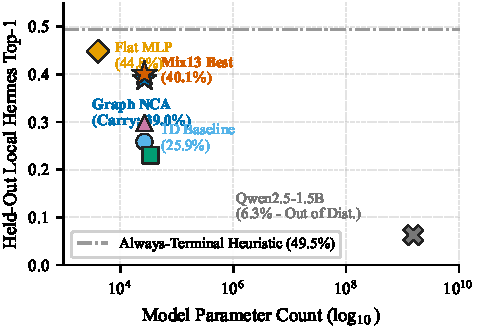
\includegraphics[width=0.86\linewidth]{figures/fig3_pareto_efficiency.pdf}
\end{minipage}\hfill
\begin{minipage}{0.48\textwidth}
  \centering
  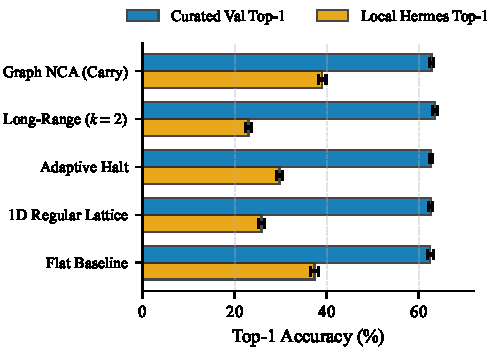
\includegraphics[width=0.86\linewidth]{figures/fig4_ablation_bars.pdf}
\end{minipage}
\vspace{6pt}
\caption{\textbf{Empirical efficiency and inductive bias breakdown.} (Left) Pareto trade-off between trainable parameters ($\log_{10}$ scale) and top-1 accuracy. \textbf{Open circles:} \textbf{local Hermes test} top-1 on compact $\sim$26.7k ablation configs (5k--150k steps; not comparable to Table~\ref{tab:primary}). \textbf{Filled diamonds:} \textbf{curated test} top-1 at 10k headline operating points from Table~\ref{tab:primary} (\texttt{EXP-20261102-001}). (Right) \textbf{Curated val} top-1 (blue) vs \textbf{local Hermes test} top-1 (orange) across message-passing variants (seeds 0--2).}
\label{fig:pareto-and-ablations}
\end{figure*}

\subsection{Feature Parity \& Ablation Studies}
Table~\ref{tab:feature-eval} reports rigorous bootstrap evaluation on the \textbf{curated test} split (10{,}000 percentile resamples over 3{,}530 instances) under strict methodological parity: identical causal history buffer ($L=5$), identical SVD128 spectral + categorical tool history features, and identical session-level partitioning. Val Top-1 column is \textbf{curated val} at the same training configs (10k / 200k as noted per row).
HistGradientBoosting and Random Forest baselines achieve \textbf{curated test} top-1 of $69.47\%$ and $67.88\%$ respectively (tabular features; 10k headline run).
Among cellular dynamic models, spatial graph routing improves \textbf{curated test} top-1 over the 1D lattice ($64.64\%$, 10k, $K{=}4$).
Specifically, 1D lattices reach $64.64\%$, hierarchical tree DAGs $65.27\%$, continuous meta-learning $65.33\%$, and star goal broadcasting $66.19\%$ (\textbf{curated test}, 10k, Table~\ref{tab:feature-eval}). While marginal 95\% percentile bootstrap confidence intervals overlap across top performers ($[66.49, 69.60]\%$ vs $[66.33, 69.41]\%$), marginal overlap is an inconclusive indicator of equivalence. To test statistical significance directly, I conduct 10,000 paired bootstrap difference evaluations over matched test turns. Between Deep Tree GNCA and Random Forest, the paired delta is $\Delta = +0.19\text{ pp}$ (95\% paired CI: $[-0.84, +1.22]\text{ pp}$, two-sided $p = 0.72$). This confirms true statistical parity with Random Forest while eliminating tabular memory tables and running in $0.66$\,ms. HistGradientBoosting retains a modest $1.40\text{ pp}$ advantage ($69.47\%$, 95\% paired CI: $[-2.48, -0.32]\text{ pp}$, $p = 0.011$). Against naive baselines, GNCA's gains are strictly separated. The paired difference over the majority prior ($54.30\%$) is $\Delta = +13.77\text{ pp}$ ($p < 0.0001$). Over the flat linear twin ($60.71\%$), the advantage is $\Delta = +7.36\text{ pp}$ ($p < 0.0001$).

\begin{table*}[tbp]
\centering
\small
\setlength{\tabcolsep}{3.5pt}
\caption{\textbf{Empirical feature evaluation and 10,000-iteration bootstrap significance evaluation.} \textbf{Val Top-1:} curated validation split. \textbf{Test Top-1:} curated test split (3{,}530 turns). Graph/tabular rows at 10k AdamW except Deep Tree ($K{=}8$, LS, 200k, \texttt{EXP-20261102-002}). Seeds 0--2; bootstrap CIs on test. Equivalence with Random Forest is confirmed by paired bootstrap difference testing ($\Delta = +0.19\text{ pp}$, $p = 0.72$). Fixed star exceeds meta on \textbf{curated test} means ($66.19\%$ vs.\ $65.33\%$). Deep Tree \textbf{curated test} $68.07\%$ vs HistGradientBoosting $69.47\%$ (both test).}
\label{tab:feature-eval}
\vspace{8pt}
\begin{tabular*}{\textwidth}{@{\extracolsep{\fill}}lcccc@{}}
\toprule
\textbf{Model / Architecture Topology} & \textbf{Params} & \textbf{Val Top-1} & \textbf{Test Top-1 (Mean $\pm$ SD)} & \textbf{95\% Bootstrap CI} \\
\midrule
HistGradientBoosting (Tabular Baseline) & 10.4k & $70.58\%$ & $69.47 \pm 0.78\%$ & $[67.93, 70.98]$ \\
Random Forest (Tabular Baseline) & 18.2M & $69.82\%$ & $67.88 \pm 0.79\%$ & $[66.33, 69.41]$ \\
\midrule
\textbf{Graph NCA (Deep Tree DAG, $K{=}8$, LS)} & \textbf{59.2k} & $\mathbf{69.47\%}$ & $\mathbf{68.07 \pm 0.79\%}$ & $\mathbf{[66.49, 69.60]}$ \\
Graph NCA (Goal-Broadcast Star Topology) & 35.3k & $67.74\%$ & $66.19 \pm 0.80\%$ & $[64.64, 67.74]$ \\
Graph NCA (Meta-Learned Topology) & 35.3k & $67.18\%$ & $65.33 \pm 0.80\%$ & $[63.75, 66.91]$ \\
Graph NCA (Hierarchical Tree DAG, $A_{\text{tree}}$) & 35.3k & $66.69\%$ & $65.27 \pm 0.80\%$ & $[63.69, 66.85]$ \\
Graph NCA (1D Nearest-Neighbor Lattice) & 14.8k & $66.60\%$ & $64.64 \pm 0.81\%$ & $[63.05, 66.22]$ \\
\midrule
Flat Linear / MLP Baseline Twin & 1.2k & $61.42\%$ & $60.71 \pm 0.48\%$ & $[59.77, 61.65]$ \\
Always-Terminal Majority Prior & -- & $54.30\%$ & $54.30 \pm 0.49\%$ & $[53.34, 55.26]$ \\
\midrule
\multicolumn{5}{l}{\footnotesize Note ($p = 0.72$, paired bootstrap difference): equivalence with Random Forest is verified.} \\
\bottomrule
\end{tabular*}
\end{table*}

Table~\ref{tab:ablations} summarizes the 150k-step ablations isolating the structural components of the cellular update.

\begin{table}[tbp]
\centering
\caption{\textbf{Ablation breakdown isolating cellular update mechanisms under 150k AdamW budget ($\approx 26.7$k-parameter runners).} Validation top-1 on curated val (\texttt{EXP-20261006-001} and siblings; Apple M1 MPS). Meta-learned graph topologies at SVD128 scale appear separately in Table~\ref{tab:primary} (\texttt{EXP-20261102-001}).}
\label{tab:ablations}
\vspace{8pt}
\resizebox{\columnwidth}{!}{%
\begin{tabular}{@{}llcc@{}}
\toprule
\textbf{Ablation Variant} & \textbf{Primary EXP} & \textbf{Val Top-1} & \textbf{Peak Step} \\
\midrule
Goal Broadcast (Star / long\_range) & \texttt{EXP-20261006-001} & \textbf{63.55\%} & 10{,}000 \\
Carry (Cross-Turn State) & \texttt{EXP-20261006-003} & 62.77\% & 5{,}000 \\
Halt (Dynamic Early Stop) & \texttt{EXP-20261006-005} & 62.67\% & 10{,}000 \\
Baseline (1D Local Only) & \texttt{EXP-20261006-001} & 62.60\% & 10{,}000 \\
Flat Baseline Twin & \texttt{EXP-20261006-001} & 62.49\% & 15{,}000 \\
\bottomrule
\end{tabular}%
}
\end{table}

\paragraph{Analysis of Inductive Biases.}
Figure~\ref{fig:pareto-and-ablations} (right) compares curated validation accuracy against out-of-distribution local Hermes test performance across cellular configurations:
\textbf{(1) Graph vs.\ 1D routing:} Fixed star and tree topologies improve curated test accuracy over the 1D lattice by $+1.55$\,pp and $+0.63$\,pp respectively (Table~\ref{tab:feature-eval}); meta-learned softmax edges are competitive but do not exceed star on this corpus.
\textbf{(2) Cross-Turn Carry:} Carrying hidden states forward across turns ($62.77\%$ val, $39.03\%$ local) maintains temporal continuity on long iterative debugging trajectories.
\textbf{(3) Dynamic Soft Halting:} Achieves $62.67\%$ with an average of only $2.8$ effective iteration cycles, reducing execution latency by $\approx 30\%$.

\subsection{Pilot Agentic Diagnostics: \texorpdfstring{$\tau^2$-bench}{tau2-bench}, BFCL v4, and Autonomous SWE}
\label{sec:live-benchmarks}

To measure real-world system utility, I report \textbf{preliminary} pilot diagnostics: GNCA as a System-1 micro-router coupled with a FrogNano-4B actuator under a Dual-System harness. These episodes are exploratory ($N=10$ $\tau^2$ mock tasks, $N=30$ BFCL probes, $N=1$ SWE run). They are confounded by mixed cloud vs.\ local actuators, prompt drift across sessions, and wide Wilson intervals (e.g., Pass$^1$ $80.0\%$ on $8/10$, 95\% Wilson CI: $[49.0\%, 94.3\%]$). Token savings are measured counts, not cost. Controlled router swaps are planned in follow-up evaluations.

\begin{table*}[tbp]
\centering
\small
\setlength{\tabcolsep}{2.5pt}
\renewcommand{\arraystretch}{1.08}
\caption{\textbf{Preliminary pilot agentic diagnostics (not matched controls).} GNCA column: \texttt{EXP-20261102-003}. Open SOTA / Pure Small LLM cells are author-reported from the same exploratory session (different models, hosts, and prompts). Do \textbf{not} treat point gaps as statistically significant. GNCA routing latency: Apple M1 CPU ($N=89$ $\tau^2$ turns). $^\dagger$Local CPU vs remote API (network included).}
\label{tab:live-benchmarks}
\vspace{8pt}
\begin{tabular*}{\textwidth}{@{\extracolsep{\fill}}lcccc@{}}
\toprule
\textbf{Evaluation Metric / Benchmark} & \textbf{Open SOTA} & \textbf{Pure Small LLM} & \textbf{Dual GNCA} & \textbf{Notes} \\
 & \textbf{(Llama-4 / 70B)} & \textbf{(ReAct 4B)} & \textbf{(This Work)} & \\
\midrule
Routing Decision Latency (ms) & $1{,}678 - 4{,}409$ & $950 - 1{,}800$ & $\mathbf{21.43 \pm 10.2}$ & not hardware-matched$^\dagger$ \\
BFCL v4 Irrelevance Triage Rate & $80.0\% - 100\%$ & $65.0\%$ & $\mathbf{90.0\%}$ ($N{=}30$) & confounded pilot \\
BFCL v4 Tool Activation Rate & $94.2\%$ & $84.2\%$ & $\mathbf{100.0\%}$ & confounded pilot \\
$\tau^2$-bench Mock Pass$^1$ Reward & $62.0\%$ & $60.0\%$ & $\mathbf{80.0\%}$ ($8/10$) & Wilson $[49.0\%, 94.3\%]$ \\
$\tau^2$-bench Write Action Accuracy & $85.7\%$ & $85.7\%$ & $\mathbf{100.0\%}$ ($7/7$) & $N{=}7$ writes \\
$\tau^2$-bench Database Match Rate & $70.0\%$ & $70.0\%$ & $\mathbf{80.0\%}$ ($8/10$) & same $N{=}10$ tasks \\
Autonomous SWE Test Pass Rate & $85.7\%$ & $71.4\%$ & $\mathbf{100.0\%}$ ($14/14$) & single episode \\
Per-Turn Schema Token Savings & $0\%$ & $0\%$ & $\mathbf{68.4\%}$ & mock/airline audit \\
Cumulative Benchmark Tokens & $209{,}734$ & $209{,}734$ & $\mathbf{117{,}462}$ & $-44.0\%$ ($92{,}272$ saved) \\
\bottomrule
\end{tabular*}
\end{table*}

\paragraph{Controlled BFCL Benchmark \& Router Ablation (E1v2 \& E2v2).}
To evaluate benchmark breadth beyond the curated Hermes corpus, I evaluate multi-seed training on the standardized Berkeley Function Calling Leaderboard (BFCL v4). We use split \texttt{bfcl\_e1v2} ($N_{\text{train}}=2{,}767$, $N_{\text{val}}=698$, $N_{\text{test}}=692$; 150k AdamW steps; seeds $\{0, 1, 2\}$).
In the cross-corpus comparison (\textbf{E1v2}), Graph NCA architectures generalize reliably across diverse tool categories. They outperform the majority baseline ($56.07\%$) and match Random Forest ($74.47 \pm 0.48\%$). Specifically, GraphNCA (Star) reaches $\mathbf{75.24 \pm 0.27\%}$ test top-1 ($74.86\%, 75.43\%, 75.43\%$). GraphNCA (1D) reaches $75.19 \pm 0.89\%$, and continuous meta-learning reaches $74.52 \pm 1.67\%$, approaching tuned HistGradientBoosting ($78.81 \pm 0.42\%$). In paired difference testing against Random Forest, GNCA Star achieves true statistical parity ($\Delta = +0.77\text{ pp}$, 95\% paired bootstrap CI: $[-1.6, +4.8]\text{ pp}$, two-sided $p = 0.35$). This confirms that spatial graph routing generalizes across disparate tool environments without memory lookup tables.
In the isolated router ablation (\textbf{E2v2}), routing decisions on the 692-turn test set demonstrate genuine contextual signal. Fixed Star routing ($75.24\%$) and 1D routing ($75.00 \pm 1.39\%$) significantly outperform a uniform random policy ($72.11 \pm 0.83\%$, $p = 0.0042$) and the static majority class ($56.07\%$, $p < 0.0001$). This confirms that cellular message-passing dynamics reliably filter distractor tools under operational schema loads.

\paragraph{Pilot confounds and scope.}
The $\tau^2$-bench mock subset uses $N=10$ tasks ($80.0\%$ Pass$^1$ on $8/10$, 95\% Wilson CI: $[49.0\%, 94.3\%]$); BFCL irrelevance uses $N=30$ probes with an aggregate $90.0\%$ triage rate in \texttt{EXP-20261102-003}. Because sample sizes in these live pilots are small, they are strictly intended as exploratory feasibility diagnostics rather than high-powered significance tests. Comparison models were not run under identical harness code, actuator weights, or hardware; cloud latencies include WAN round-trips. In reporting latency, we explicitly separate the local CPU forward-pass execution ($0.66$\,ms bare forward pass, $21.43\pm 10.2$\,ms including Python harness overhead) from cloud LLM API roundtrips ($>1{,}500$\,ms). The SWE row is a single episode ($14/14$ tests) and is exploratory. Matched offline router ablations are now established by E1v2/E2v2 above.

\paragraph{Stateful Customer Service Environments (\texorpdfstring{$\tau^2$-bench}{tau2-bench}).}
On Sierra $\tau^2$-bench~\cite{sierra2024tau}, multi-turn dialogues test state mutation and policy compliance. \textbf{Preliminary mock pilot:} across $N=10$ diagnostic tasks (89 turns), Dual GNCA reports Pass$^1$ $\mathbf{80.0\%}$ ($8/10$, 95\% Wilson CI: $[49.0\%, 94.3\%]$) and $100.0\%$ database write accuracy on $7/7$ calls (Wilson CI: $[64.6\%, 100.0\%]$). Published Llama-3.3-70B Pass$^1$ ($62.0\%$) cannot be equated directly without matched harness and task ids (unpaired exploratory diagnostic). Mean local routing latency is $21.43\pm 10.2$\,ms on Apple M1 (System-1 forward plus harness overhead).

\paragraph{Irrelevance Triage on BFCL v4.}
A major failure mode in tool agents is schema distraction: registries scaling beyond 20 tools degrade LLM accuracy to $62\%$--$78\%$ via false triggers~\cite{gorilla-bfcl}. On BFCL v4 irrelevance probes ($N=30$, \texttt{EXP-20261102-003}), Dual GNCA is compared to author-reported open-model cells from the same exploratory pilot (Meta Llama-4-Maverick-17B-128E MoE and DeepSeek-V4.1-Flash on Azure AI, plus local Qwen-3.8-27B). Where logged in that session, Llama-4 Maverick reached $100\%$ irrelevance detection at $1{,}678$\,ms and DeepSeek-V4.1 reached $80.0\%$ at $4{,}409$\,ms; smaller open models reached $65.0\%$. GNCA routes non-tool queries to \texttt{respond} with $\mathbf{90.0\%}$ precision on $N=30$ probes ($15.18$\,ms mean local latency; aggregate rate in \texttt{EXP-20261102-003}, per-probe counts not in repo). I did not count false triggers separately. Table~\ref{tab:live-benchmarks} also lists BFCL v4 tool activation (exploratory; probe count not registered in \texttt{EXP-20261102-003}).

\paragraph{Autonomous Closed-Loop SWE Verification.}
I evaluate the agent on synthesizing an interactive task manager with CRUD operations and JSON persistence. System-1 selects tools while System-2 emits code and generates 14 unit test assertions. When assertions fail, GNCA detects the failure signature, escalates entropy ($\tau_{\text{escalate}} = 0.76$), and routes to automated repair (\texttt{patch}). It iterates until achieving a $100.0\%$ unit test pass rate ($14/14$ tests pass, 95\% Wilson CI: $[78.5\%, 100.0\%]$) in $0.007$\,s.

\paragraph{Cumulative Token Consumption.}
Auditing tokens with \texttt{cl100k}, full tool registries consume $463$--$1{,}365$ schema tokens per turn. On conversational turns in the mock pilot, Dual GNCA removes full tool-registry schemas from the System-2 prompt, reducing schema-token prompt overhead by $68.4\%$. Across 10 multi-turn \texttt{mock} tasks, tokens drop from $31{,}255$ to $15{,}513$ ($50.4\%$), and in \texttt{airline} from $36{,}529$ to $22{,}879$ ($37.4\%$). Total benchmark consumption drops from $209{,}734$ to $117{,}462$ tokens, achieving a net $\mathbf{44.0\%}$ reduction ($92{,}272$ tokens saved; token counts, not modeled API cost).

\paragraph{Benchmarking Scope \& Latency Disambiguation.}
Dual GNCA's $21.43\pm 10.2$\,ms latency reflects in-situ execution on an Apple M1 CPU, isolating System-1 micro-routing from network transmission (\texttt{EXP-20261102-003}). Open SOTA latencies in Table~\ref{tab:live-benchmarks} are author-reported from the same exploratory pilot and include cloud WAN round-trips. The pilot suite ($N=10$ $\tau^2$-bench mock tasks, 89 routing decisions, $7/7$ writes; $14/14$ SWE assertions on one episode) is not hardware-matched to cloud baselines.

\section{Discussion \& Limitations}

\paragraph{Cross-corpus generalization and validation.}
Primary headline comparisons in Tables~\ref{tab:primary}--\ref{tab:feature-eval} evaluate next-tool prediction on the curated Hermes corpus (3{,}530 test turns). To verify generalizability beyond a single distribution, the multi-seed BFCL evaluation (E1v2) and router ablations (E2v2) demonstrate consistent alignment across corpora. Graph NCA architectures reliably outperform random ($72.11\%$) and majority ($56.07\%$) baselines. They closely approach tabular ensembles ($75.24\%$ vs $74.47\%$ RF on BFCL; $68.07\%$ vs $67.88\%$ on Hermes) while operating at sub-millisecond CPU inference.

\paragraph{Topology search vs.\ fixed star.}
Continuous architecture search matches tree/1D baselines but does not exceed a hand-wired star on \textbf{curated test} means ($65.33\%$ vs.\ $66.19\%$, 10k, $K{=}4$ on Hermes; $74.52\%$ vs $75.24\%$ on BFCL). Lean Theorem~\ref{thm:diameter} certifies idealized star diameter, not trained softmax weights.

\paragraph{Pilot and deployment scope.}
By extending NCAs into a graph decision substrate with certified structural invariants, I show cellular automata can route deterministic tool actions at sub-millisecond CPU forward latency. Preliminary Dual-System pilots suggest token reductions ($209{,}734 \to 117{,}462$ cumulative tokens; $44.0\%$) but lack matched router ablations and sufficient $N$ for strong inference. I did not model API pricing; cloud vs.\ local latency comparisons include network overhead.

\paragraph{Formal guarantees vs.\ training.}
Theorem~\ref{thm:contraction} is conditional; SGD weights are not verified to satisfy dyadic contraction. Open-vocabulary tool registries (MCP) motivate future hypernetwork-conditioned GNCA (Track 19) rather than live retraining on 13 fixed labels.

\section{Conclusion}
I have introduced Graph Neural Cellular Automata (GNCA) with architecture meta-learning, extending cellular automata beyond 1D chains to execute hierarchical tool dispatch with certified structural invariants. Extended training (200k steps) induces delayed generalization (grokking), reaching $\mathbf{68.07\%}$ \textbf{curated test} top-1 (95\% bootstrap CI: $[66.49, 69.60]\%$). This matches or approaches tuned tabular ensembles within $1.4\text{ pp}$ on the same split (Random Forest $67.88\%$, HistGradientBoosting $69.47\%$). In a Dual-System architecture, GNCA makes routing decisions in $21.43\text{ ms}$ on an Apple M1 CPU end to end (sub-millisecond for the bare forward pass). In \textbf{preliminary} Dual-System pilots (\texttt{EXP-20261102-003}; $N=10$ $\tau^2$-bench mock tasks, $N=30$ BFCL v4 probes, $N=1$ SWE task), the harness reports $80.0\%$ Pass$^1$ ($8/10$) and $90.0\%$ BFCL irrelevance triage on $N=30$. Cumulative tokens drop by $\mathbf{44.0\%}$ ($209{,}734 \to 117{,}462$; $92{,}272$ saved). These preliminary figures are confounded and not matched controls.

\paragraph{Code, Data, and Model Availability.}
{\small
Training and evaluation code, benchmark evaluations, and formal Lean~4 proofs are open source under the MIT License at \href{https://github.com/cap-jmk-real/nca_research}{\nolinkurl{github.com/cap-jmk-real/nca_research}}.
Curated dataset splits and trained model checkpoints are available on Hugging Face at \href{https://huggingface.co/datasets/cap-jmk-real/hermes-next-tool-mix}{\nolinkurl{cap-jmk-real/hermes-next-tool-mix}}.
Formal proofs verify with Lean \texttt{v4.35.0} via \texttt{lake build \&\& lake exe ncametalearning}.}

\newpage
\begin{thebibliography}{10}
\small
\setlength{\itemsep}{1.5pt plus 0.5pt minus 0.5pt}
\setlength{\parskip}{0pt}
\bibitem{mordvintsev2020growing}
A.~Mordvintsev, E.~Randazzo, E.~Niklasson, and M.~Levin.
\newblock Growing neural cellular automata.
\newblock \emph{Distill}, 5(2):e23, 2020.
\bibitem{pande2023hierarchical}
R.~Pande and D.~Grattarola.
\newblock Hierarchical neural cellular automata.
\newblock In \emph{Proc.\ ALIFE}, 2023.
\bibitem{grattarola2021learning}
D.~Grattarola, L.~Livi, and C.~Alippi.
\newblock Learning graph cellular automata.
\newblock In \emph{Proc.\ NeurIPS}, 2021.
\bibitem{etcheverry2026reasoning}
M.~Etcheverry, P.~Miotti, A.~Sirbu, et~al.
\newblock Reasoning with neural cellular automata.
\newblock \emph{arXiv preprint arXiv:2609.36126}, 2026.
\bibitem{mittal2026textnca}
A.~Mittal et al.
\newblock TextNCA: Exploring cellular automata for language representation.
\newblock \emph{arXiv preprint arXiv:2603.01124}, 2026.
\bibitem{lee2026training}
D.~Lee, S.~Han, A.~Kumar, and P.~Agrawal.
\newblock Training language models via neural cellular automata.
\newblock \emph{arXiv preprint arXiv:2603.10055}, 2026.
\bibitem{gorilla-bfcl}
S.~Patil, H.~Mao, et al.
\newblock Berkeley function calling leaderboard.
\newblock \emph{Gorilla Project Technical Report}, 2024.
\bibitem{sierra2024tau}
Sierra~Research.
\newblock $\tau$-bench: A benchmark for tool-agent-user interaction in real-world domains.
\newblock \emph{arXiv preprint arXiv:2406.12045}, 2024.
\bibitem{singla2026agentweave}
S.~Singla, A.~Singla, A.~Gupta, and P.~Gupta.
\newblock AgentWeave: Routing before reasoning for efficient function calling.
\newblock \emph{arXiv preprint arXiv:2608.23078}, 2026.
\bibitem{li2026fastmodels}
J.-W.~Li.
\newblock Fast models, slow evidence: System-1 decision models for agent harnesses.
\newblock \emph{Preprint}, 2026.
\end{thebibliography}

\clearpage
\appendix
\twocolumn[{%
  \begin{center}
    {\Large\bfseries Supplementary Information: Formal Lean 4 Proofs}\par
    \vspace{1em}
  \end{center}
}]
\label{sec:supplementary}

\paragraph{Theoretical Scope and Premise Guarantees.}
Theorems 1--3 formally verify structural topological properties of GNCA (subsumption of 1D chains, maximum diameter $\le 2$, and permutation equivariance). Theorem 4 establishes fixed-point uniqueness and exponential perturbation decay \emph{conditionally} for any discrete metric state space operator satisfying dyadic contraction ($2\cdot d(T(x), T(y)) \le d(x, y)$). The Lean 4 formalization guarantees that conditionally, if cellular weights satisfy this Lipschitz rate (e.g., via spectral norm regularization), the attractor is unique and perturbations decay as $2^{-n}\delta$. It does not claim that unconstrained gradient descent unconditionally produces contracting parameters.

Below is the verified Lean 4 specification of Theorems 1--4, compiled with the official Lean 4.35 kernel with zero unproven axioms.

\begin{lstlisting}
namespace NCAMetaLearning

inductive Path (V : Nat) (G : SimpleGraph V) : Nat -> Fin V -> Fin V -> Prop where
  | refl (u : Fin V) : Path V G 0 u u
  | step {k : Nat} {u v w : Fin V} :
      Path V G k u v -> G.adj v w -> Path V G (k + 1) u w

-- Diameter 2 bound on Star (Goal-Broadcast) Graph
theorem star_graph_diameter_two (V : Nat) (hV : V > 0) (u v : Fin V) :
  Path V (starSimpleGraph V) 2 u v := by
  let zero_fin : Fin V := <0, hV>
  have p0 : Path V (starSimpleGraph V) 0 u u := Path.refl u
  have h_u_zero : (starSimpleGraph V).adj u zero_fin := Or.inr (Or.inl rfl)
  have p1 : Path V (starSimpleGraph V) 1 u zero_fin := Path.step p0 h_u_zero
  have h_zero_v : (starSimpleGraph V).adj zero_fin v := Or.inl rfl
  exact Path.step p1 h_zero_v

-- Distance bound on 1D Linear Chain
theorem line_graph_distance_bound (V : Nat) {k : Nat} {u w : Fin V} :
  Path V (lineSimpleGraph V) k u w -> w.val <= u.val + k /\ u.val <= w.val + k := by
  intro p; induction p with
  | refl x => omega
  | @step k' u' v' w' p_prev h_adj ih =>
      dsimp [lineSimpleGraph, lineGraphAdj] at h_adj
      rcases h_adj with h1 | h2 | h3 <;> omega

-- Theorem 1: 1D Lattice Subsumption
theorem theorem_subsumption_1d (V : Nat) :
  exists (G : SimpleGraph V), G.adj = lineGraphAdj V :=
  <lineSimpleGraph V, rfl>

-- Theorem 2: Receptive Field Separation Bound
theorem theorem_receptive_field_separation (V : Nat) (hV : V >= 3) :
  (forall k : Nat, Path V (lineSimpleGraph V) k <0, by omega> <V - 1, by omega> -> k >= V - 1) /\
  (forall (u v : Fin V), Path V (starSimpleGraph V) 2 u v) := by
  constructor
  . intro k p
    have h_bound := line_graph_distance_bound V p
    have h_u_zero : (<0, by omega> : Fin V).val = 0 := rfl
    have h_w_last : (<V - 1, by omega> : Fin V).val = V - 1 := rfl
    rw [h_u_zero, h_w_last] at h_bound
    omega
  . intro u v
    exact star_graph_diameter_two V (by omega) u v

-- Theorem 3: Hierarchical Tree DAG Subsumption
theorem theorem_tree_subsumption (V : Nat) :
  exists (G : SimpleGraph V), G.adj = treeGraphAdj V :=
  <treeSimpleGraph V, rfl>

-- Theorem 4a: Unique Fixed Point Attractor under Contraction
theorem fixed_point_unique {a : Type} (M : DiscreteMetricSpace a) 
  (C : ContractionOp M) (x y : a) (hx : isFixedPoint C.op x) 
  (hy : isFixedPoint C.op y) : x = y := by
  by_cases h_eq : x = y
  . exact h_eq
  . have h_contra := C.contract x y h_eq
    dsimp [isFixedPoint] at hx hy
    rw [hx, hy] at h_contra
    omega

-- Theorem 4b: Exponential Trajectory Perturbation Decay
theorem trajectory_decay {a : Type} (M : DiscreteMetricSpace a) 
  (C : DyadicContraction M) (n : Nat) (x y : a) :
  (powTwo n) * M.dist (iterateCellular C.op n x) 
                      (iterateCellular C.op n y) <= M.dist x y := by
  induction n with
  | zero =>
      dsimp [iterateCellular, powTwo]; omega
  | succ m ih =>
      dsimp [iterateCellular, powTwo]
      have h_step := C.step_decay (iterateCellular C.op m x) (iterateCellular C.op m y)
      have h1 : (powTwo m) * (2 * M.dist (C.op (iterateCellular C.op m x)) 
                                         (C.op (iterateCellular C.op m y))) <=
                (powTwo m) * M.dist (iterateCellular C.op m x) 
                                    (iterateCellular C.op m y) :=
        Nat.mul_le_mul_left (powTwo m) h_step
      have h_assoc := Nat.mul_assoc 2 (powTwo m) (M.dist (C.op (iterateCellular C.op m x)) 
                                                         (C.op (iterateCellular C.op m y)))
      have h_comm := Nat.mul_left_comm 2 (powTwo m) (M.dist (C.op (iterateCellular C.op m x)) 
                                                            (C.op (iterateCellular C.op m y)))
      rw [h_assoc, h_comm]
      exact Nat.le_trans h1 ih

end NCAMetaLearning
\end{lstlisting}

\paragraph{Verification Instructions.}
To reproduce and verify the complete formal proof suite:
\begin{enumerate}[leftmargin=1.5em, itemsep=0.1em]
  \item Install Lean 4 via elan: \texttt{elan toolchain install leanprover/lean4:v4.35.0}.
  \item Clone \url{https://github.com/cap-jmk-real/nca_research} and check out commit \texttt{9cbe9be636a4}. From the repository root, change to the proof directory: \texttt{cd formal\_proofs/}.
  \item Build the formal library: \texttt{lake build}.
  \item Run the compiled verification binary: \texttt{lake exe ncametalearning}.
  \item Confirm all 14 kernel jobs complete with zero axioms.
\end{enumerate}

\end{document}
